\section{Question 2}
        \subsection{a}
            Sufficient schedulability test for RM scheduling: $U <= n(2^{1/n} - 1)$ \\ where n is the number of tasks in the task set and U is the processor utilization factor, $U = \sum_{i=1}^{n} \frac{C_i}{T_i}$. 

        \renewcommand{\arraystretch}{1.4}
        \begin{figure}[H]
        \centering
        \begin{minipage}{0.5\textwidth}
            \begin{table}[H]
            \centering
            \begin{tabular}{|l|l|l|}
                \hline
                \textbf{Task}   & \textbf{T=D}  & \textbf{C}  \\ \hline
                A               & 3             & 1           \\ \hline
                B               & 5             & 2           \\ \hline
                C               & 2             & 0.5         \\ \hline

            \end{tabular}
            \end{table}
        \end{minipage}%
        \caption{Task set}
        \label{fig:Taskset}
        \end{figure}
    \renewcommand{\arraystretch}{1.0}

        \subsubsection{Task set schedulable?}
        $U = \sum_{i=1}^{n} \frac{C_i}{T_i} = \frac{1}{3} + \frac{2}{5} + \frac{0.5}{2} = 0.98$ \\
        $U <= n(2^{1/n} - 1) = 3(2^{1/3} - 1) = 0.78$ \\
        Since the statement $U <= n(2^{1/n} - 1)$ is false in this case, the task set cannot be proven to be schedulable with this sufficient test method.

        \subsection{b}
            \subsubsection{Exact schedulability test, Tracing}
            \begin{figure}[H]
                \centering
                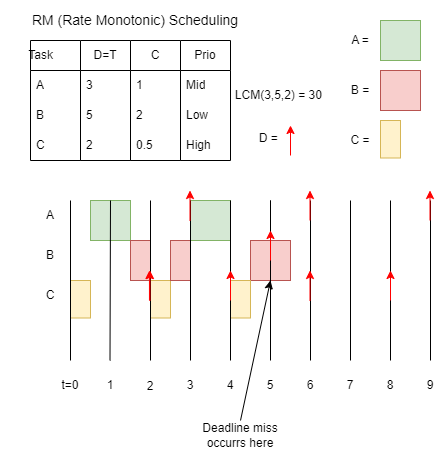
\includegraphics[width=0.5\textwidth]{images/Ass1Q2.drawio.png}
                \caption{Tracing of the task set proves that it is not schedulable with RM.}
                \label{fig:tracing}
            \end{figure}

        As demonstrated in figure above, the task set is not schedulable with RM scheduling. The task set is not schedulable because task B misses its deadline at $t = 5$.
